\documentclass {article}
\usepackage{amsmath} % paquete de matemáticas
\usepackage{xtab} % paquete de tablas
\usepackage{graphicx} % paquete de graficas
\usepackage{subfigure} % paquete de figuras
\usepackage{fullpage} % paquetes para utilizar toda la pagina
\usepackage{blindtext} % paquete para texto de relleno 
\usepackage{hyperref}

\author{Ana Laura Sarracino Ortiz}
\date{Mon, Jul 4$^{\text {th }}$}
\pagestyle{empty}

\title{\sc Ecuaciones, tablas y figuras}


\begin{document}

\maketitle{}	
\thispagestyle{empty}

\blindtext
\\

\vspace{1cm}
En la Fig. (\ref{fig:reproduccion}) se observa el proceso de reproducci\'on de la lombriz de tierra Eisenia foetida y en la Fig. (\ref{fig:alimentacion}) la forma de alimentaci\'on mediante la degradac\'ion de residuos org\'anicos.

\begin{figure}{r}[h!b] % lenguaje para insertar una imagen
  \vspace{-20pt}
  \begin{center}
    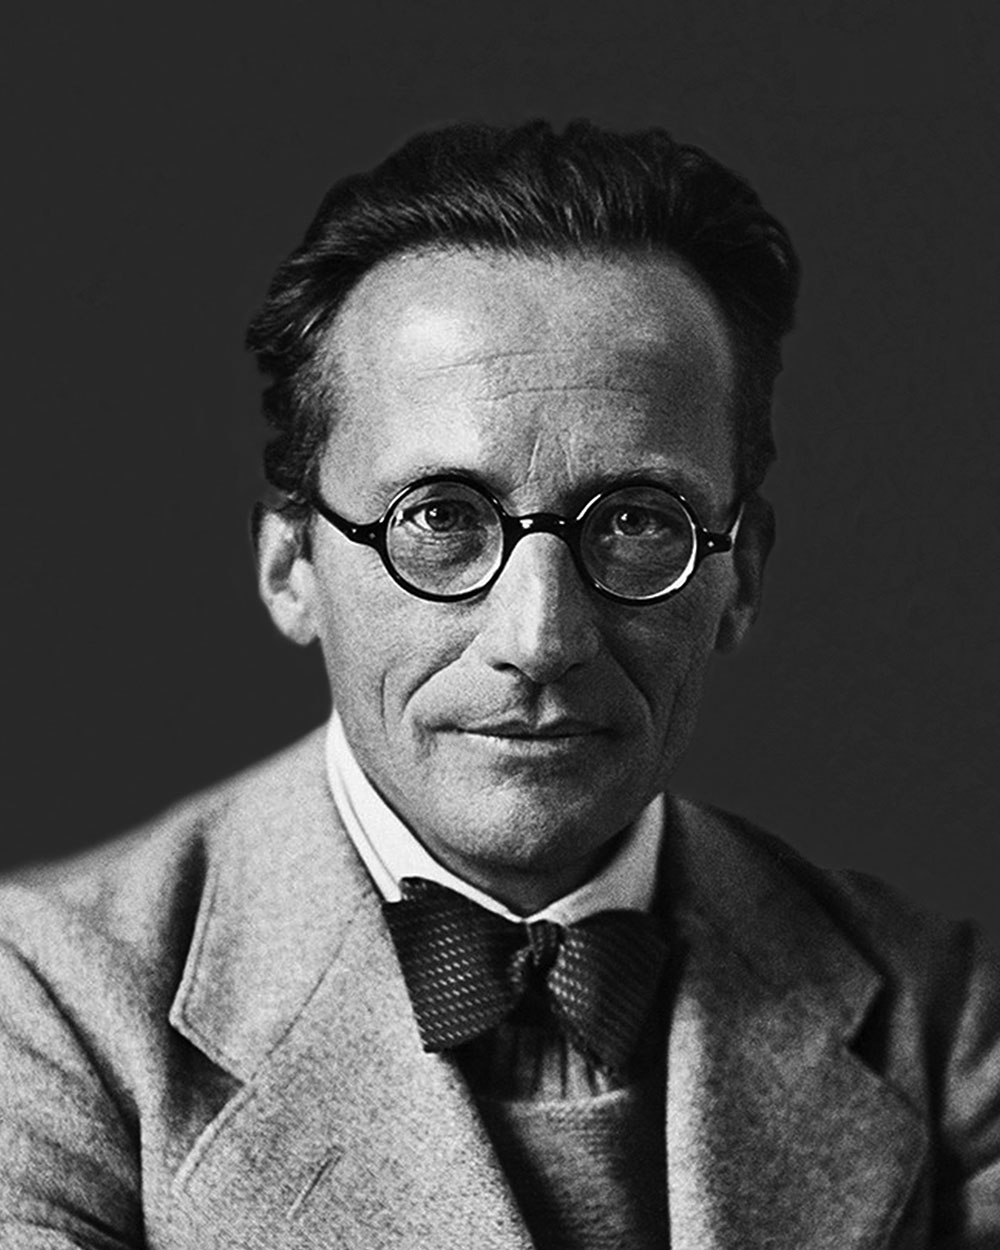
\includegraphics[width=0.48\textwidth]{Erwin}
  \end{center}
  \vspace{-20pt}
  \caption{A gull}
  \vspace{-10pt}
	\centering
	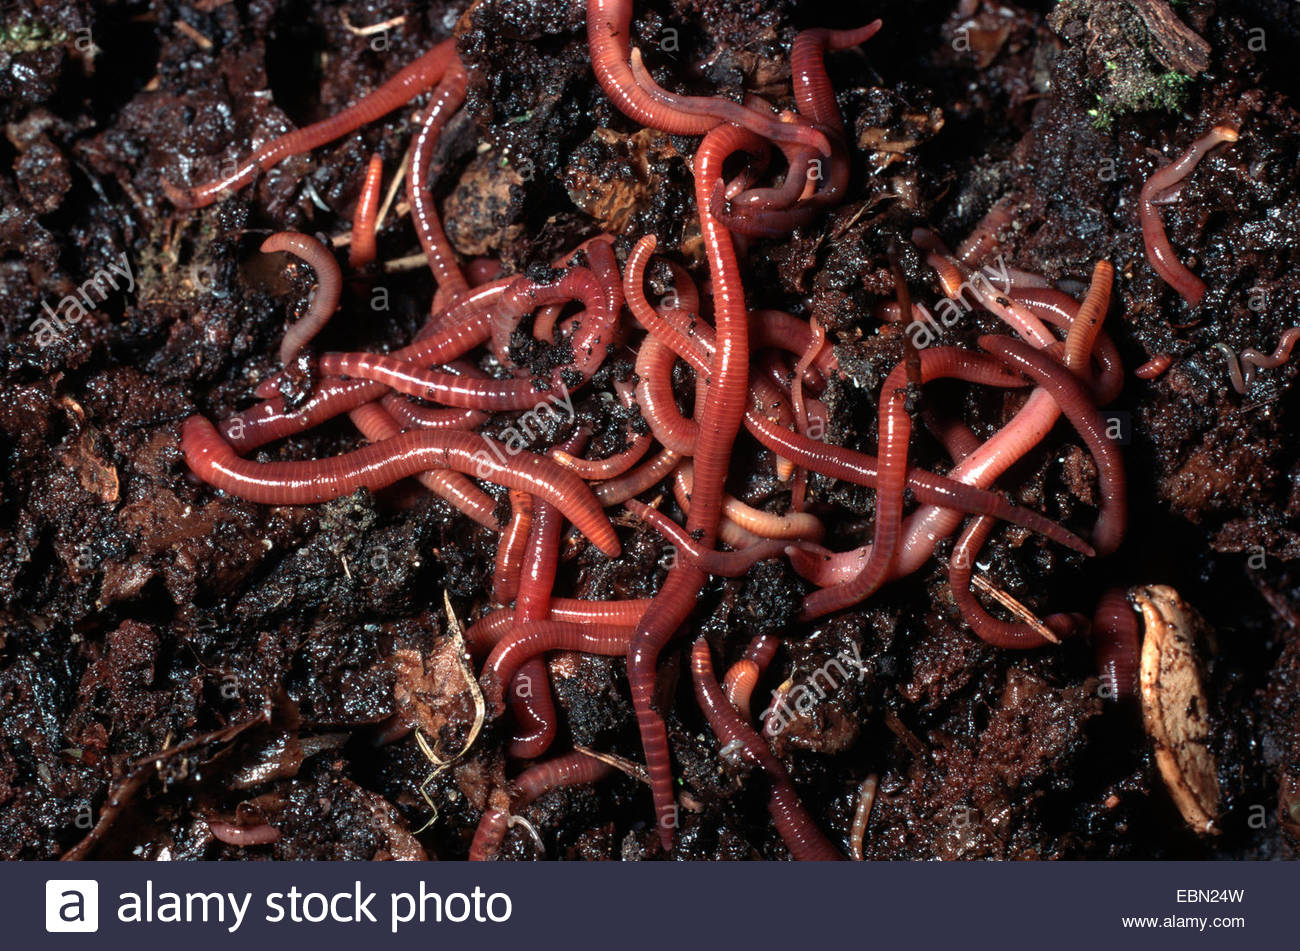
\includegraphics[width=0.3\textwidth]{vectorial} \\ % ancho de la figura o tamaño
	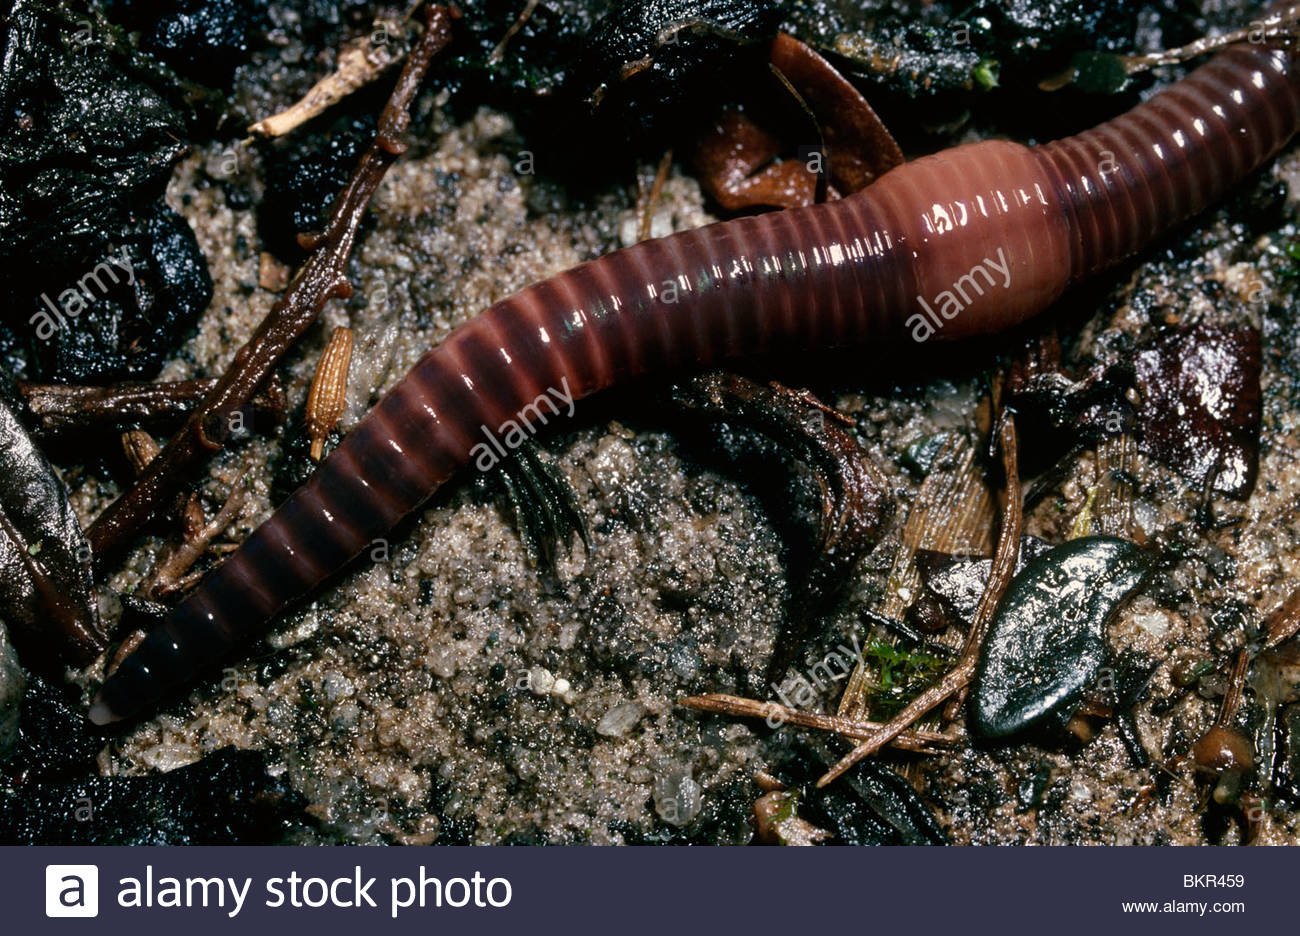
\includegraphics[width=0.3\textwidth]{vectorial2}
	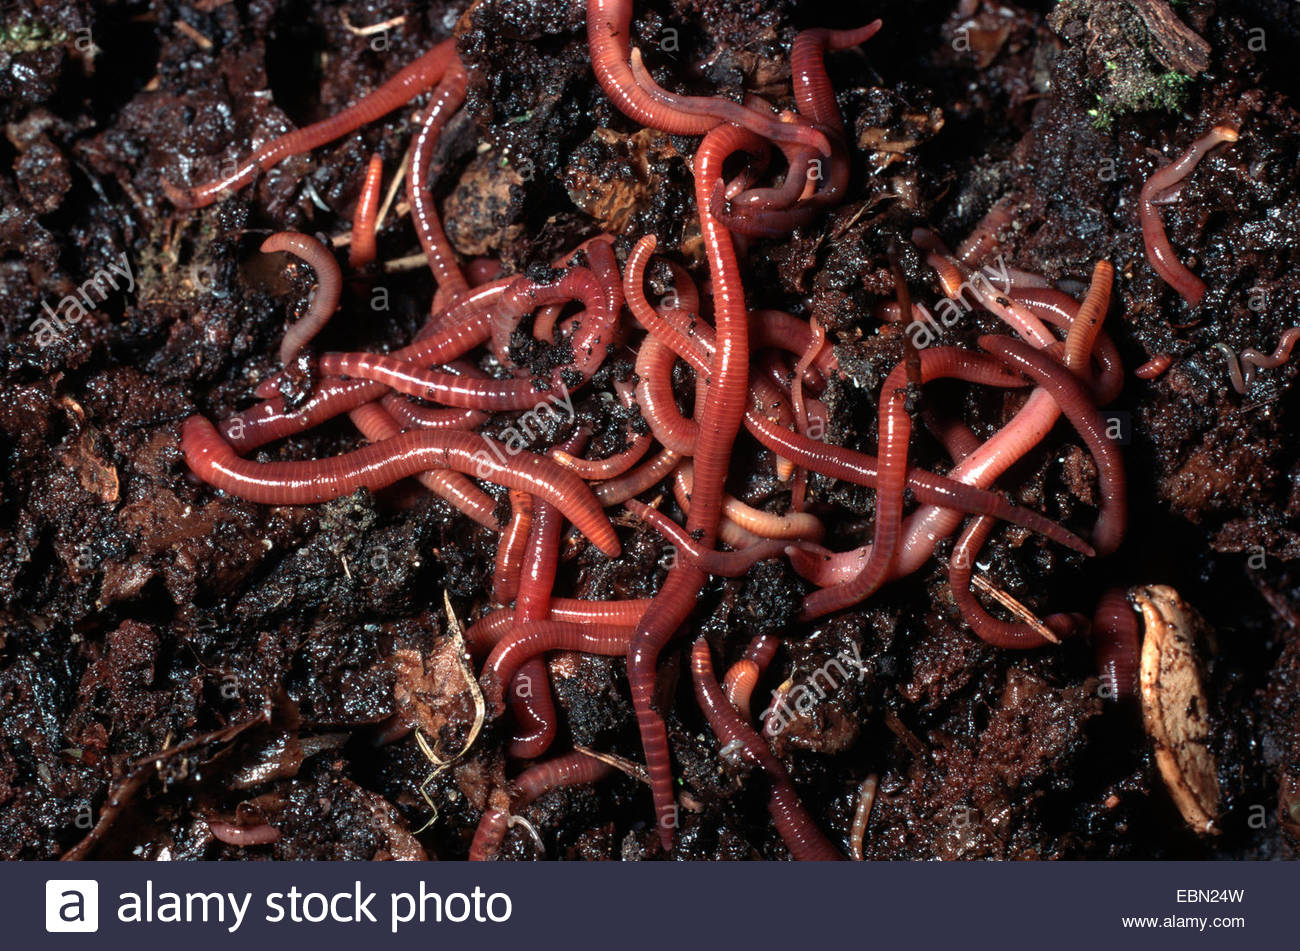
\includegraphics[width=0.3\textwidth]{vectorial}
	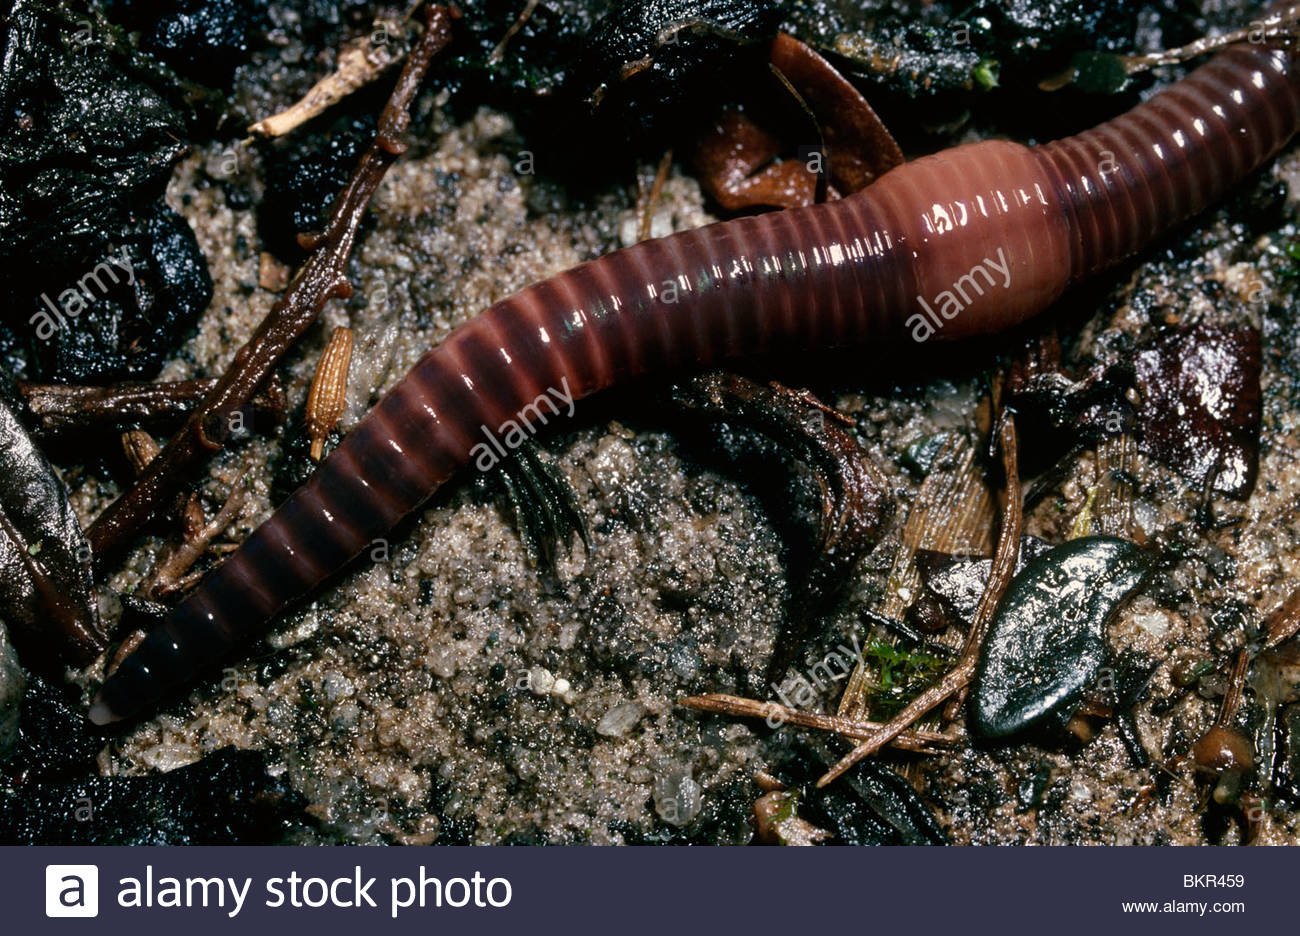
\includegraphics[width=0.3\textwidth]{vectorial2} % se repite este comando para colocar dos imagenes de forma horizontal
	\caption{Reproducci\'on de lombriz de tierra.} % pie de figura
	\label{fig:reproduccion} % solo poner una palabra que nos recuerdde a la figura y hacer la cita de forma rapida
\end{figure}{wrapfigure}

\begin{figure}[h!]
	\centering
	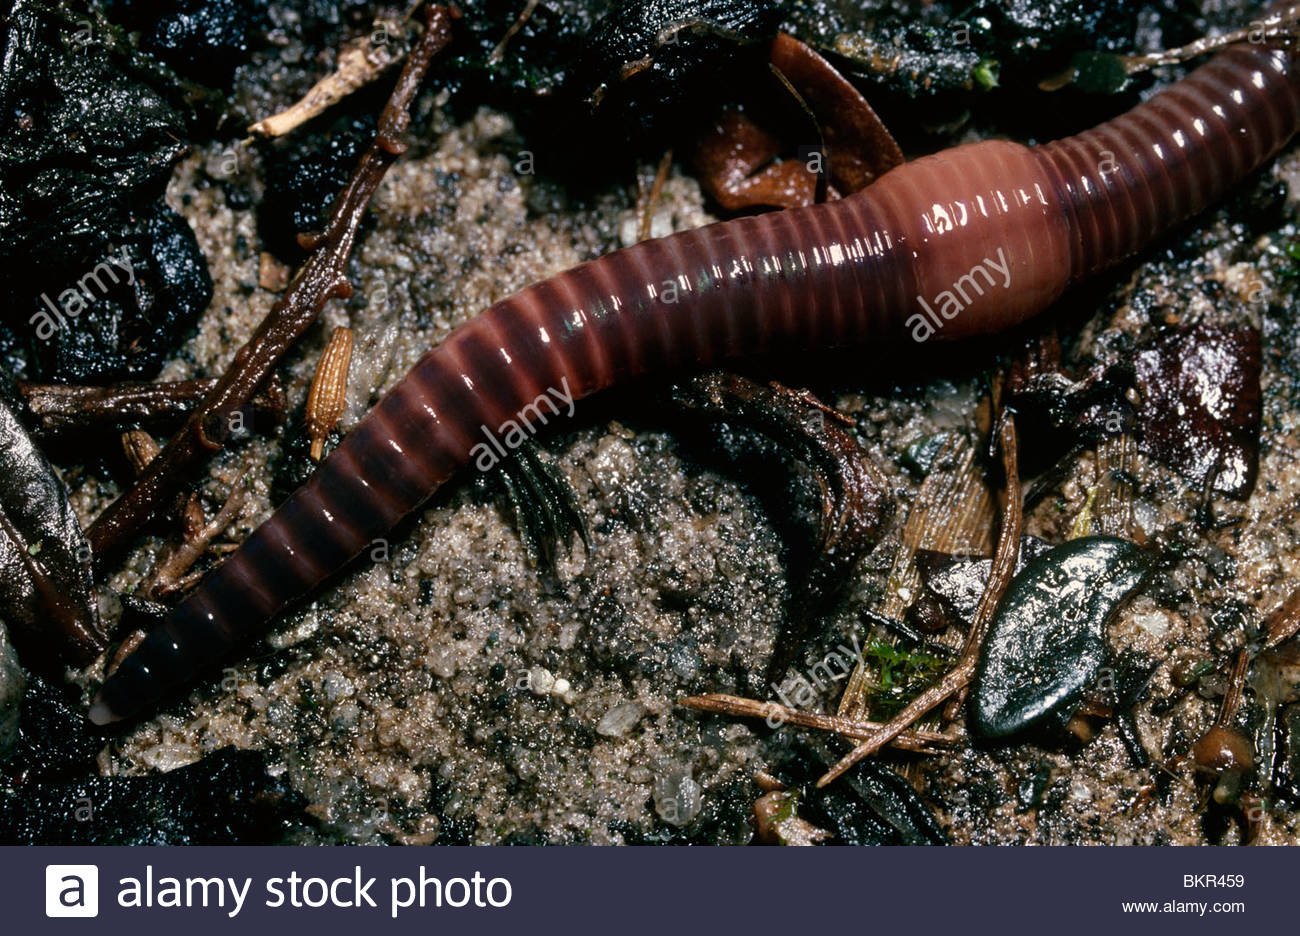
\includegraphics[width=0.3\textwidth]{vectorial2}
	\caption{Degradaci\'on de residuos org\'anicos}
	\label{fig:alimentacion}
\end{figure}

Para m\'as informaci\'on acerca de figuras visitar  \href{https://en.wikibooks.org/wiki/LaTeX/Floats,_Figures_and_Captions}{este v\'inculo}

\section{Equations} % (fold)
\label{sec:equations}

Como se vio en la secci\'on \ref{sec:equations}uno se pueden citar distintos entornos como figuras y ecuaciones (Eq. \eqref{sec:equations})

\begin{equation}
pi*r{^2}
\end{equation}



\section{Tabular}
\label{sec:tabular}

\begin{tabular}{|l|c|r|}

\hline
\hline
\textbf{Nombre} & \textbf{Edad} & \textbf{Estado}\\
\hline
\hline
Ana     & 24 & Tabasco\\
Marcela & 21 & Tabasco\\
Gullermo& 24 & Querétaro\\

\end{tabular}

\end{document}































